\documentclass[12pt]{article}

\usepackage{sbc-template}

\usepackage{graphicx,url}

\usepackage[utf8]{inputenc}  

%Portuguese-specific commands
%--------------------------------------
\usepackage[portuguese]{babel}
%--------------------------------------

%Hyphenation rules
%--------------------------------------
\usepackage{hyphenat}
%--------------------------------------
\usepackage{minted}

\sloppy

\title{Árvore de van Emde Boas: Explicação e Implementação}

\author{Leandro Gabriel, Walter F. Siqueira}


\address{Instituto de Computação - Universidade Federal Fluminense (UFF)\\
  Niterói - RJ - Brazil
  \email{\{leandrogabriel,waltersiqueira\}@id.uff.br}
}

\begin{document} 

\maketitle

\begin{abstract}
  This paper describes the data structure applied in van Emde Boas trees and shows examples of dynamic queries, including examples of these operations and a presentation of data organization step-by-step in them.
\end{abstract}
     
\begin{resumo} 
  Este artigo descreve a estrutura de dados aplicada na árvore de van Emde Boas e apresenta exemplos de operações de conjunto dinâmico, além de uma representação da organização dos dados passo a passo em tais operações.
\end{resumo}


\section{Introdução} \label{sec:intro}

Este artigo descreve a estrutura de dados aplicada na árvore de van Emde Boas e apresenta exemplos de operações de conjunto dinâmico, além de uma representação da organização dos dados passo a passo em tais operações.

De acordo com [CORMEN 2012], nas estruturas de dados que suportam as operações de uma fila de prioridades - isto é, heaps binários, árvores vermelho-preto e heaps de Fibonacci -, no mínimo uma operação importante demora O(lg n), seja do pior caso, seja amortizado. No caso das árvores de van Emde Boas, é possível explorar informações adicionais sobre as chaves para ordenar no tempo o(n lg n), com a desvantagem de que as chaves precisam ser um inteiro na faixa 0 a n-1, e sem duplicatas.

É suportado pelas árvores de van Emde Boas todas as operações de conjunto dinâmico, isto é, SEARCH, INSERT, DELETE, MINIMUM, MAXIMUM, SUCCESSOR e PREDECESSOR, todas no pior tempo O(lg lg n). Devido a elas se basearem em chaves e não permitir chaves duplicadas, a operação SEARCH pode ser implementada como a operação MEMBER(S, x), que é mais simples e retorna um booleano que indica se o valor x está atualmente no conjunto dinâmico S.

\section{Abordagens preliminares} \label{sec:abordagensPreliminares}

Antes de prosseguirmos para o entendimento da árvore de van Emde Boas, precisamos compreender duas abordagens: sobrepor uma estrutura de árvore binária de bits em um vetor, e sobrepor uma árvore de altura constante - ou, árvore de grau.

Para estas abordagens, podemos realizar o endereçamento direto, pois é a abordagem mais simples para armazenar um conjunto dinâmico. Aqui, trataremos o conjunto dinâmico como um vetor de bits $A[0..u-1]$, de $u$ bits, onde $A[x]$ contém 1 se o valor de x estiver no conjunto dinâmico. Caso contrário, contém 0.

\subsection{Sobrepondo árvore binária de bits}

Nesta abordagem, tratamos as entradas do vetor de bits como as folhas da árvore. os nós pais armazenam o bit referente à operação lógica OR (OU) de seus dois filhos, até sua raiz. Deste modo, os nós contém 1 se e somente se qualquer forma em sua subárvore contém 1, assim como representado na figura~\ref{fig:arvoreBinariaBits}.

\begin{figure}[ht]
\centering
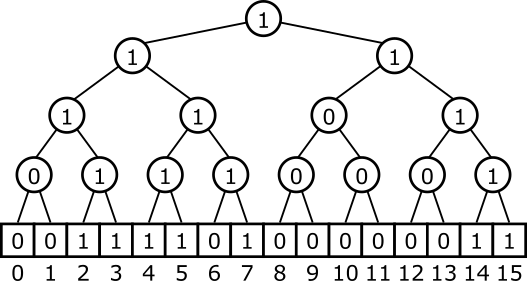
\includegraphics[width=0.7\textwidth]{arvoreBinariaBits.png}
\caption{Vetor de bits sobreposto por uma árvore binária de bits}
\label{fig:arvoreBinariaBits}
\end{figure}

Neste caso, as operações que levavam o tempo $\Theta(u)$ do pior caso com um vetor de bits agora usam a estrutura de árvore. O caminho a se percorrer para cada uma das operações é:
\begin{itemize}
    \item MININUM: Da raiz às folhas, sempre buscando o nó à extrema esquerda que possui 1;
    \item MAXIMUM: Da raiz às folhas, sempre buscando o nó à extrema direita que possui 1;
    \item SUCCESSOR: De x à raiz, até entrar em um nó pela esquerda e este nó tiver 1 à direita. Caso positivo, desce por ele, sempre buscando o nó à extrema esquerda que possui 1;
    \item PREDECESSOR: De x à raiz, até entrar em um nó pela direita e este nó tiver 1 à esquerda. Caso positivo, desce por ele, sempre buscando o nó à extrema direita que possui 1;
    \item INSERT: Armazena 1 em x, e segue até a raiz executando a operação lógica OU no nó pai, referente à presença dos filhos;
    \item DELETE: Armazena 0 em x, e segue até a raiz executando a operação lógica OU no nó pai, referente à presença dos filhos.
\end{itemize}

Como resultado, cada uma destas operações demoram $O(lg\ u)$ no pior caso, visto que a altura da árvore é $lg\ u$ e cada uma das operações executam no máximo uma passagem ascendente pela árvore e no máximo uma passagem descendente. De acordo com [CORMEN 2012], isto faz com que ela seja marginalmente melhor do que as árvores vermelho-preto, pois MEMBER é executada no tempo $O(1)$ e, se $n$ for muito menor que $u$, a árvore vermelho-preto será mais rápida para todas as outras operações.

\subsection{Sobrepondo árvore de grau (altura constante)}

A árvore de altura constante possui sua quantidade de elementos igual à raiz quadrada de $u$. Neste caso, é chamada árvore de grau $\sqrt{u}$. A figura~\ref{fig:arvoreAlturaConstante} representa que os elementos x do conjunto dinâmico fazem parte de um subconjunto de $\sqrt{u}$ elementos - denominado \textbf{cluster} -, que será referenciado pelo índice da árvore de altura constante. A este vetor chamamos de ''sumário'' pois o valor de cada índice é a operação lógica OU de todos os elementos de seu cluster.

\begin{figure}[ht]
\centering
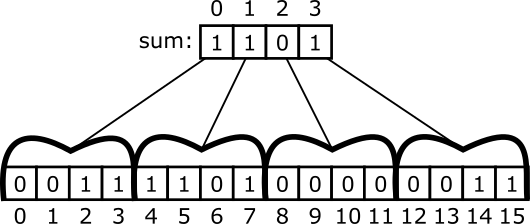
\includegraphics[width=0.7\textwidth]{arvoreAlturaConstante.png}
\caption{Vetor de bits sobreposto por uma árvore de grau $\sqrt{u}$}
\label{fig:arvoreAlturaConstante}
\end{figure}

Para esta árvore, as operações funcionam da seguinte maneira:
\begin{itemize}
    \item MINIMUM: No sumário, da extrema esquerda que possui 1, buscando dentro do i-ésimo cluster para o 1 à extrema esquerda deste;
    \item MAXIMUM: No sumário, da extrema direita que possui 1, buscando dentro do i-ésimo cluster para o 1 à extrema direita deste;
    \item SUCCESSOR: De x, procura 1 à sua direita, dentro de seu cluster. Caso não encontre, sobe ao sumário e busca o próximo 1 à direita. Ao encontrar, busca dentro do i-ésimo cluster para o 1 à extrema esquerda deste;
    \item PREDECESSOR: De x, procura 1 à sua esquerda, dentro de seu cluster. Caso não encontre, sobe ao sumário e busca o próximo 1 à esquerda. Ao encontrar, busca dentro do i-ésimo cluster para o 1 à extrema direita deste;
    \item INSERT: Define 1 em $A[x]$ e em $sum[x/\sqrt{u}]$. Aqui, a operação é resolvida em $O(1)$;
    \item DELETE: Define 0 em $A[x]$ e define em $sum[x/\sqrt{u}]$ a operação lógica de todo o cluster.
\end{itemize}

Como resultado, cada uma destas operações, exceto INSERT, são resolvidas em $O(\sqrt{u})$. [CORMEN 2012] relata que não há progresso no uso dessa abordagem pois, sobrendo uma árvore binária, as operações eram resolvidas em $O(lg\ u)$, que é assintoticamente mais rápido que $O(\sqrt{u})$.

\section{van Emde Boas} \label{sec:vanEmdeBoas}

A árvore de van Emde Boas foi idealizada pelo doutor informática neerlandês Peter \textbf{van Emde Boas}, em 1975. Trata-se de uma árvore binária cuja estrutura permite que cada uma das operações de ocnjunto dinâmico sejam executadas no pior tempo O(lg lg n).

Comumente denotada como $vEB$, a base dos elementos de um nó da árvore é a faixa de valores possíveis - aqui, chamada de ''universo'' -, representada por $u$. Deste modo, $u$ é uma potência exata de 2, isto é, $u = 2^{k}$, onde $k$ é a chave de um determinado nó. O tempo de execução do pior caso de cada uma das operações é $O(lg\ lg\ u)$.

Contudo, a estrutura de uma $vEB$ exige que as chaves sejam números inteiros na faixa de $0$ a $n-1$, sem duplicatas. Por serem chaves, as $vEB$ não possuem a operação SEARCH, e sim MEMBER(S, x), que retorna um booleano indicando se o valor x está no conjunto dinâmico S.

A prototipação da $vEB$ é aqui denominada como $proto-vEB$. Nela, van Emde Boas prototipou que fosse armazenado um nó de sumário, além dos clusters, assim como representado na figura~\ref{fig:protovEB}. Apesar de funcional, a $proto-vEB$ não alcança $O(lg\ lg\ u)$ pois ainda executava recursão muitas vezes na maioria das operações.

\begin{figure}[ht]
\centering
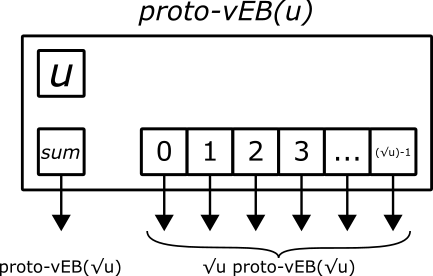
\includegraphics[width=0.7\textwidth]{protovEB.png}
\caption{Representação do conteúdo de um nó $proto-vEB$}
\label{fig:protovEB}
\end{figure}

Para se evitar a maioria de tais recursões, foram implementados também dois campos para armazenar a chave mínima e máxima de cada nó, conforme a figura~\ref{fig:vEB}. Esta é a representação da própria $vEB$, contendo todos os elementos necessários para efetuar as operações em $O(lg\ lg\ u)$

\begin{figure}[ht]
\centering
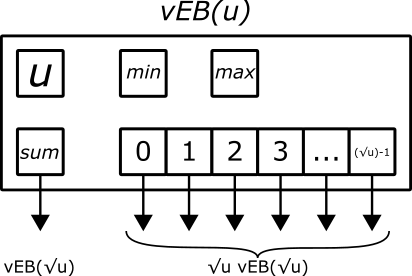
\includegraphics[width=0.7\textwidth]{vEB.png}
\caption{Representação do conteúdo de um nó $vEB$}
\label{fig:vEB}
\end{figure}

Os sumários das $vEB$ dentro dos clusters auxiliam a $vEB$ pai na obtenção dos resultados das operações. Para sua estrutura, uma $vEB$ precisa saber o tamanho de seu ''universo''. A raiz quadrada deste universo é repassada como o tamanho de seu cluster, e define também o tamanho do universo de cada $vEB$ filha, através do teto desse valor. Uma $vEB$ com um universo de 2 índices não possui sumário nem cluster, e sim apenas as informações de valor mínimo e máximo. A figura~\ref{fig:vEB(4)} representa uma árvore vEB com um universo de 4 chaves.

\begin{figure}[ht]
\centering
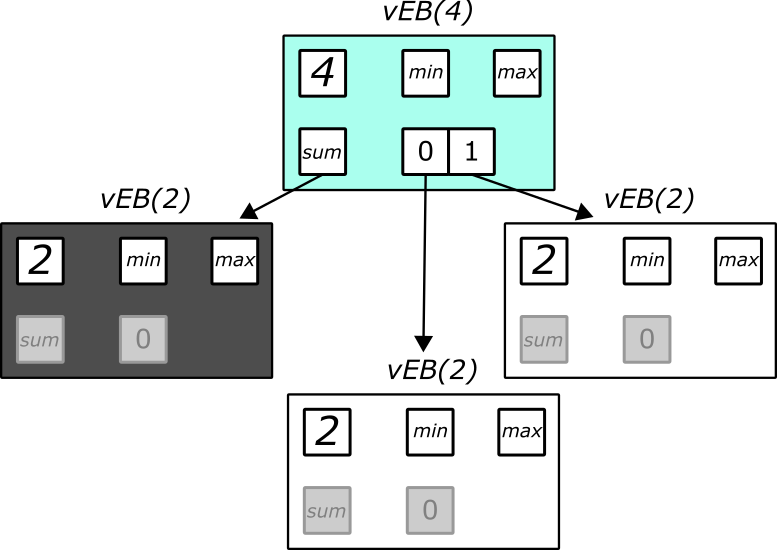
\includegraphics[width=0.7\textwidth]{vEB(4).png}
\caption{Uma estrutura $vEB(4)$. Note que a raiz é composta por mínimo, máximo, um $vEB$ sumário e dois $vEB$, que são seus clusters. Todos os seus filhos (incluindo o sumário, em cor escura), por serem $u=2$, possuem apenas as informações de mínimo e máximo.}
\label{fig:vEB(4)}
\end{figure}

Como resultado, cada uma das operações da $vEB$ é capaz de operar em $O(1)$ no melhor tempo. No pior tempo, em $O(lg\ lg\ u)$. Contudo, é necessário um maior espaço em memória para armazenar a árvore. Além disto, caso a $vEB$ trabalhe com poucos elementos, existem alternativas melhores, visto que a criação de uma árvore vazia executa no tempo $O(u)$. Para que seja possível essa criação, ao criar sua raiz, é necessário saber quantos elementos terá no universo da mesma. Finalizando, os valores de uma $vEB$ precisam ser números inteiros, sem duplicatas.

\section{Implementação da $vEB$}

Faremos a implementação a seguir utilizando a linguagem javascript, para que seja possível visualizar uma representação desta implementação em uma página na internet. Os códigos aqui demonstrados estão disponíveis em \url{http://github.com/leo150250/vanemdeboas}.

\subsection{Classe $vEB$}
Por padrão, um nó $vEB$ possuirá -1 como min e max, não terá sumario nem clusters. Este -1 é o mesmo que dizer que ''não há'' um valor, isto é, é ''vazio''. Contudo, para que seja possível criar este nó de acordo com as especificações de uma $vEB$, seu método construtor exige que seja informado o tamanho do universo deste nó.
\begin{minted}[frame=lines,breaklines]{javascript}
class Van_Emde_Boas {
    universo=-1;
    min=-1;
    max=-1;
    sumario=null;
    clusters=[];
    (...)
}
\end{minted}
O método construtor terá, portanto, um argumento obrigatório, e utilizará o valor deste argumento para fazer os cálculos e gerar os seus possíveis sumários e clusters. Caso o tamanho do universo deste nó seja 2 ou menor, então aqui encerra a execução deste nó. Caso contrário, então obtém-se o número de clusters através da fórmula matemática $\lceil \sqrt{u} \rceil$ e usa este resultado para criar, recursivamente, o sumário e os $\lceil \sqrt{u} \rceil$ clusters, colocando o tamanho do universo deles sendo $\lceil \sqrt{u} \rceil$.
\begin{minted}[frame=lines,breaklines]{javascript}
class Van_Emde_Boas {
    (...)
    constructor(argTamanho) {
        this.universo = argTamanho;
        this.min = -1;
        this.max = -1;
        if (this.universo <= 2) {
            this.sumario = null;
            this.clusters[0] = null;
        } else {
            let numClusters = Math.ceil(Math.sqrt(this.universo));
            this.sumario = new Van_Emde_Boas(numClusters);
            for (let i = 0; i < numClusters; i++) {
                this.clusters[i] = new Van_Emde_Boas(numClusters);
            }
        }
    }
    (...)
}
\end{minted}

\subsection{Métodos das chaves}
Como as $vEB$ não armazenam seu valor final e sim chaves para que possam ser utilizadas em operações matemáticas a fim de auxiliar no retorno dos valores, precisamos de métodos a fim de auxiliar na busca por tais chaves. Estes métodos, no padrão denominados high(x), low(x) e key(x,y), aqui são implementados como obterPai(x), obterFilho(x) e gerarChave(x,y), para fins didáticos.

O método obterPai(x) retorna um valor inteiro da fórmula $x / \lceil \sqrt{u} \rceil$. Já o método obterFilho(x) retorna um valor inteiro da fórmula $x \bmod{\lceil \sqrt{u} \rceil}$.
\begin{minted}[frame=lines,breaklines]{javascript}
class Van_Emde_Boas {
    (...)
    obterPai(argChave) {
        let div = Math.ceil(Math.sqrt(this.universo));
        return parseInt(argChave / div);
    }
    obterFilho(argChave) {
        let mod = Math.ceil(Math.sqrt(this.universo));
        return argChave % mod;
    }
    (...)
}
\end{minted}

Para se descobrir o valor de uma determinada chave, é necessário dois argumentos, pois o resultado será $x * \lceil \sqrt{u} \rceil + y$. Esta fórmula permite retornar a posição da chave a partir de sua posição no cluster y e do índice do cluster x.
\begin{minted}[frame=lines,breaklines]{javascript}
class Van_Emde_Boas {
    (...)
    gerarChave(argPai, argFilho) {
        return argPai * Math.ceil(Math.sqrt(this.universo)) + argFilho;
    }
    (...)
}
\end{minted}

Para obter o mínimo e o máximo de um determinado nó, podemos utilizar os valores que estão registrados nas variáveis min e max. Isto já faz com que tais operações sejam executadas em, na maioria das vezes, no tempo $O(1)$. Em javascript não há necessidade mas, caso queira utilizar uma função para retornar estes valores ou, esteja desenvolvendo com encapsulamento (o que não é o caso aqui), elas seriam da seguinte forma:
\begin{minted}[frame=lines,breaklines]{javascript}
class Van_Emde_Boas {
    (...)
    definirMin(argMin) {
        this.min=argMin;
    }
    definirMax(argMax) {
        this.max=argMax;
    }
    obterMin() {
        return this.min;
    }
    obterMax() {
        return this.max;
    }
    (...)
}
\end{minted}

\subsection{Operações de busca}
Por serem chaves, as $vEB$ possuem a função MEMBER, aqui implementada como verificar(x). Ela retorna um booleano, e aqui foram implementados alguns casos para auxiliar no processamento, onde:
\begin{itemize}
    \item Caso o universo seja menor que a chave procurada, então retorna-se \textbf{falso} pois, nessa implementação, o tamanho do universo pode ser quaisquer potências de 2;
    \item Caso min ou max seja igual ao valor da chave procurada, então retorna-se \textbf{verdadeiro} pois a chave é um dos limites deste nó, provando que o valor está presente;
    \item Caso contrário, então provavelmente a chave deve estar em algum dos filhos. \textbf{Prossegue a busca recursivamente} para o cluster da chave (obterPai(x)) em busca da chave de sua posição neste cluster (obterFilho(x));
    \item Para haver garantia de que o código será executado caso tenha clusters disponíveis, se o cluster não existir (isto é, ''null''), então retorna \textbf{falso}.
\end{itemize}

\begin{minted}[frame=lines,breaklines]{javascript}
class Van_Emde_Boas {
    (...)
    verificar(argChave) {
        if (this.universo <= argChave) {
            return false;
        }
        if (this.min == argChave || this.max == argChave) {
            return true;
        } else {
            if (this.universo==2) {
                return false;
            } else {
                if (this.clusters[ this.obterPai(argChave) ] != null) {
                    return this.clusters[ this.obterPai(argChave) ].verificar( this.obterFilho(argChave), false, argCancelarRegistro);
                } else {
                    return false;
                }
            }
        }
    }
    (...)
}
\end{minted}

Para encontrar o sucessor de uma determinada chave, a função sucessor(x) trabalha enviando a chave principal para o nó raiz e realiza os cálculos para os filhos, caso necessário, de acordo com a chave que deve ser trazida deles. O valor retornado fará parte do cálculo da função gerarChave(x,y), o que deve retornar o número referente ao sucessor da chave. Nisto, esta função recursiva executa os seguintes casos:
\begin{itemize}
    \item Caso o universo do nó seja 2, existem a possibilidade de a chave a qual se está buscando para este nó é 0, e o max é 1. Se este for o caso, retorna 1. Caso contrário, retorna -1;
    \item Caso o nó possua um min e a chave a ser buscada é menor que ele, retorna-se o valor do min;
    \item Caso contrário, obtém o valor max do cluster pai da chave. Se houver max e o valor filho da chave for menor que ele, então prossegue recursivamente para este cluster, buscando o valor filho da chave. O valor que esta recursividade retornar é utilizado como um offset no cálculo da função gerarChave(x,y), usando x como o valor pai dessa chave e y como o valor offset;
    \item Caso contrário ao item anterior, então prossegue recursivamente para o sumario deste nó, buscando o valor pai da chave. Se o valor desta recursividade retornar -1, então não há um sucessor. Caso contrário, usa o valor como indice dos clusters deste nó para obter o min deste, e usa-o como offset no cálculo da função gerarChave(x,y), usando x como o valor retornado da recursividade e y como o valor  offset.
\end{itemize}

\begin{minted}[frame=lines,breaklines]{javascript}
class Van_Emde_Boas {
    (...)
    sucessor(argChave) {
        if (this.universo==2) {
            if ((argChave==0) && (this.max==1)) {
                return 1;
            } else {
                return -1;
            }
        } else if ((this.min!=-1) && (argChave<this.min)) {
            return this.min;
        } else {
            let clusterMaximo = this.clusters[this.obterPai(argChave)].max;
            let offsetCluster=0;
            let sucessorCluster=0;
            if ((clusterMaximo != -1) && (this.obterFilho(argChave) < clusterMaximo)) {
                offsetCluster = this.clusters[ this.obterPai(argChave) ].sucessor( this.obterFilho(argChave) );
                return this.gerarChave( this.obterPai(argChave), offsetCluster);
            } else {
                sucessorCluster = this.sumario.sucessor( this.obterPai(argChave) );
                if (sucessorCluster==-1) {
                    return -1;
                } else {
                    offsetCluster = this.clusters[ sucessorCluster ].min;
                    return this.gerarChave( sucessorCluster, offsetCluster );
                }
            }
        }
    }
    (...)
}
\end{minted}

Para encontrar o antecessor de uma determinada chave, a função antecessor(x) trabalha enviando a chave principal para o nó raiz e realiza os cálculos para os filhos, caso necessário, de acordo com a chave que deve ser trazida deles. O valor retornado fará parte do cálculo da função gerarChave(x,y), o que deve retornar o número referente ao antecessor da chave. Nisto, esta função recursiva executa os seguintes casos:
\begin{itemize}
    \item Caso o universo do nó seja 2, existem a possibilidade de a chave a qual se está buscando para este nó é 1, e o min é 0. Se este for o caso, retorna 0. Caso contrário, retorna -1;
    \item Caso o nó possua um max e a chave a ser buscada é maior que ele, retorna-se o valor do max;
    \item Caso contrário, obtém o valor min do cluster pai da chave. Se houver min e o valor filho da chave for maior que ele, então prossegue recursivamente para este cluster, buscando o valor filho da chave. O valor que esta recursividade retornar é utilizado como um offset no cálculo da função gerarChave(x,y), usando x como o valor pai dessa chave e y como o valor offset;
    \item Caso contrário ao item anterior, então prossegue recursivamente para o sumario deste nó, buscando o valor pai da chave. Se o valor desta recursividade retornar -1, se o nó tiver um min e a chave for maior que este min, então retorna o valor do min deste nó. Caso contrário, não há um antecessor. Se este não for o caso, usa o valor retornado como indice dos clusters deste nó para obter o max deste, e usa-o como offset no cálculo da função gerarChave(x,y), usando x como o valor retornado da recursividade e y como o valor  offset.
\end{itemize}

\begin{minted}[frame=lines,breaklines]{javascript}
class Van_Emde_Boas {
    (...)
    antecessor(argChave) {
        if (this.universo == 2) {
            if ((argChave == 1) && (this.min == 0)) {
                return 0;
            } else {
                return -1;
            }
        } else if ((this.max != -1) && (argChave > this.max)) {
            return this.max;
        } else {
            let clusterMinimo = this.clusters[ this.obterPai(argChave) ].min;
            let offsetCluster = 0;
            let antecessorCluster = 0;
            if ( (clusterMinimo != -1) && ( this.obterFilho(argChave) > clusterMinimo) ) {
                offsetCluster = this.clusters[ this.obterPai(argChave) ].antecessor( this.obterFilho(argChave) );
                return this.gerarChave( this.obterPai(argChave), offsetCluster);
            } else {
                antecessorCluster = this.sumario.antecessor( this.obterPai(argChave) );
                if (antecessorCluster == -1) {
                    if ((this.min != -1) && (argChave > this.min)) {
                        return this.min;
                    } else {
                        return -1;
                    }
                } else {
                    offsetCluster = this.clusters[ antecessorCluster ].max;
                    return this.gerarChave( antecessorCluster, offsetCluster );
                }
            }
        }
    }
    (...)
}
\end{minted}

\subsection{Operações de inserção e exclusão}

Para se inserir um valor em uma vEB, é realizado uma série de verificações antes de prosseguir recursivamente. As etapas são:
\begin{itemize}
    \item Se não houver min (-1 em min), é o mesmo que não haver chave neste nó. Então, define-se o valor de min e max para o valor da chave.
    \item Caso contrário, prossegue para inserção. Antes da inserção, verifica se o valor da chave é menor que o min. Se sim, inverte-se os valores.
    \item Se o universo deste nó for maior que 2, então verifica se existe min no cluster pai da chave. Se sim, prossegue recursivamente no sumário, inserindo o valor pai da chave, e atualiza o min e o max do cluster pai da chave com o valor filho da chave. Se não, prossegue recursivamente no cluster pai da chave, inserindo o valor filho da chave.
    \item Por último, se o valor da chave for maior que o max, atualiza o valor de max para o valor da chave.
\end{itemize}

\begin{minted}[frame=lines,breaklines]{javascript}
class Van_Emde_Boas {
    (...)
    inserir(argChave) {
        if (this.min == -1) {
            this.definirMin(argChave);
            this.definirMax(argChave);
        } else {
            if (argChave < this.min) {
                let aux = this.min;
                this.definirMin(argChave);
                argChave = aux;
            }
            if (this.universo > 2) {
                if (this.clusters[ this.obterPai(argChave) ].min == -1) {
                    this.sumario.inserir( this.obterPai(argChave) );
                    this.clusters[ this.obterPai(argChave) ].definirMin( this.obterFilho(argChave) );
                    this.clusters[ this.obterPai(argChave) ].definirMax( this.obterFilho(argChave) );
                } else {
                    this.clusters[ this.obterPai(argChave) ].inserir( this.obterFilho(argChave) );
                }
            }
            if (argChave > this.max) {
                this.definirMax(argChave);
            }
        }
    }
    (...)
}
\end{minted}

Para excluir um valor da vEB, os seguintes passos são realizados:
\begin{itemize}
    \item Se min e max possuem o mesmo valor, então este nó possui só esta chave. Define-se os dois como -1.
    \item Senão, se o universo deste nó for 2, define o valor de min para o valor inverso da chave (0 ou 1), e o valor de max igual ao de min.
    \item Caso contrário, antes de prosseguir verifica se o valor da chave é igual ao valor de min. Se sim, obtém o indice do primeiro cluster com base no min do sumário, e armazena como valor da chave o resultado da função gerarChave(x,y), inserindo o min do sumário como x e o min do primeiro cluster como y.
    \item Em seguida, prossegue recursivamente a exclusão para o cluster pai da chave, repassando para exclusão o valor filho da chave.
    \item Se, após a exclusão recursiva, não houver mais uma chave no cluster pai da chave, então prossegue recursivamente a exclusão para o sumário, repassando para exclusão o valor pai da chave. Em seguida, se o valor da chave for igual ao max deste nó, obtém o max de seu sumário. Se não houver max no sumário, define-se o max deste nó para o mesmo valor de min. Caso contrário, define-se o valor max deste nó para o resultado da função gerarChave(x,y), repassando o max do sumário como x e o max do cluster usando o max do sumário como índice.
    \item Agora, caso cluster do pai da chave tenha min, e o valor da chave for igual ao max, define-se o max deste nó para o resultado da função gerarChave(x,y), repassando o pai da chave como x e o max do cluster pai da chave como y.
\end{itemize}

\begin{minted}[frame=lines,breaklines]{javascript}
class Van_Emde_Boas {
    (...)
    deletar(argChave) {
        if (this.max == this.min) {
            this.definirMin(-1);
            this.definirMax(-1);
        } else if (this.universo == 2) {
            if (argChave == 0) {
                this.definirMin(1);
            } else {
                this.definirMin(0);
            }
            this.definirMax(this.min);
        } else {
            if (argChave == this.min) {
                let primeiroCluster = this.sumario.min;
                argChave = this.gerarChave( primeiroCluster, this.clusters[ primeiroCluster ].min);
                this.definirMin(argChave);
            }
            this.clusters[ this.obterPai(argChave) ].deletar( this.obterFilho(argChave) );
            if (this.clusters[ this.obterPai(argChave) ].min == -1) {
                this.sumario.deletar( this.obterPai(argChave) );
                if (argChave == this.max) {
                    let maximoSumario = this.sumario.max;
                    if (maximoSumario == -1) {
                        this.definirMax(this.min);
                    } else {
                        this.definirMax( this.gerarChave( maximoSumario, this.clusters[ maximoSumario ].max) );
                    }
                }
            } else if (argChave == this.max) {
                this.definirMax( this.gerarChave( this.obterPai(argChave), this.clusters[ this.obterPai(argChave) ].max) );
            }
        }
    }
    (...)
}
\end{minted}

\section{Referências}

Cormen, T... [et al.] (2012). Algoritmos. GEN, 3ª edição

\end{document}